% Quick start guide
\documentclass{beamer}
\usetheme{metropolis} %most minimalist found until now

\title{Using Beamers}
\subtitle{This is a subtitle}
\author{Ivan Takaki Ajimura}
\institute{University of Coimbra}
\date{\today}
% University Logo
\logo{
\includegraphics[width=2.5cm]{figures/uc-logo-hor.png}} 
\begin{document}

%Insert a title page
\begin{frame}
    \titlepage
\end{frame}

% Table of Contents
\begin{frame}{Outline}
    \tableofcontents
\end{frame}

%Sections and Subsections only appear in Table of Contents
\section{Section 1}
\subsection{Subsection 1}

% Lists
\begin{frame}{Lists in beamer}
\begin{itemize}
    \item \href{https://latex-beamer.com/}{Latex Beamer Website}
    \item Second item
    \item Third item
\end{itemize}
\end{frame}

%[<+->]
\begin{frame}{Lists in beamer}
\begin{itemize}[<+->]
    \item \href{https://latex-beamer.com/}{Latex Beamer Website}
    \item Second item
    \item Third item
\end{itemize}
\end{frame}

% Multiple columns
\begin{frame}{Two columns frame in beamer}
\begin{columns}
% Column 1
\begin{column}{0.5\textwidth}
    Colors available in xcolor
\end{column}
% Column 2
\begin{column}{0.5\textwidth}
    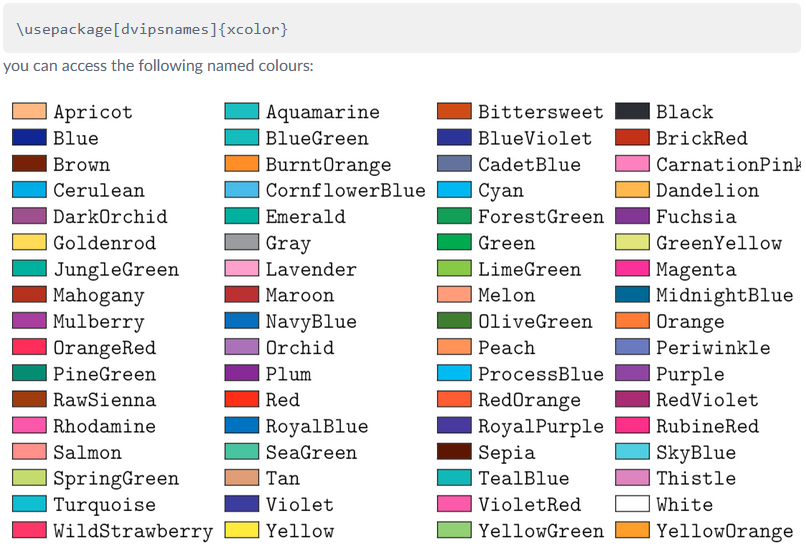
\includegraphics[scale=0.3]{figures/xcolors.png}
\end{column}
\end{columns}
\end{frame}

% Blocks
\begin{frame}{Blocks in beamer}{}
\begin{block}{Block 1}
This is a simple block in beamer.
\end{block}
\begin{alertblock}{Block 2}
This is an alert block in beamer.
\end{alertblock}
\begin{exampleblock}{Block 3}
This is an example block in beamer.
\end{exampleblock}
\begin{theorem}
    It's in \LaTeX{} so it must be true $ a^2 + b^2 = c^2$.
\end{theorem}
\begin{corollary}
    a = b
\end{corollary}
\begin{proof}
    a + b = b + c
\end{proof}
\end{frame}

% Pause command
\begin{frame}{Creating Overlays in Beamer}{Pause command}
\begin{itemize}
    \item Shown from the first slide on.
\pause
    \item Shown from the second slide on.
\pause
    \item Shown from the third slide on.
\end{itemize}
\end{frame}

% Overlays <1-3>
\begin{frame}{Creating Overlays in Beamer}{Overlay command}
\begin{itemize}
    \item<1-> Shown from the first slide on.
\pause
    \item<2-3> Shown from the second slide on.
\pause
    \item<3-> Shown from the third slide on.
\end{itemize}
\end{frame}


%onslide
 \begin{frame}{Onslide command}
This is shown on all slides.
\onslide <1-3>
\begin{itemize}
    \item This list will only be shown
    \item on slides 1, 2 and 3.
\end{itemize}
\onslide<1,4>
I appear just on slides 1 and 4.
\end{frame}


% only
\begin{frame}{Only command}
    \only<2>{\color{red}}  This text is red only on slide 2.
\end{frame}

% uncover and invisible
\begin{frame}{Uncover command}
    If you want to learn Beamer\uncover<2>{, follow latex-beamer.com!}
    
    If you want to learn Beamer\invisible<1>{, follow latex-beamer.com!}
\end{frame}


% alt
\begin{frame}{Alternative command}
    \alt<2>{We are on slide 2!}{We are not on slide 2}
\end{frame}

%Definition, example, theorem, proof, corollary
\begin{frame}{Overlay specifications Math environment}
    \begin{definition}<1->
    When something is repeated more than three times, we say it is spam
\end{definition}
\begin{example}<2->
    An example of spam is: eggs, eggs, eggs
\end{example}
\begin{theorem}<3->
    I don’t like spam!
\end{theorem}
\begin{proof}<5->
    This proof is shown after the corollary.
\end{proof}
\begin{corollary}<4->
    Spam is considered something bad
\end{corollary}
\end{frame}
\end{document}

\end{document}